\documentclass[../notes.tex]{subfiles}

\pagestyle{main}
\renewcommand{\chaptermark}[1]{\markboth{\chaptername\ \thechapter\ (#1)}{}}
\setcounter{chapter}{8}

\begin{document}




\chapter{Selection Rules and Exam}
\section{Electronic Spectroscopy: Selection Rules}
\begin{itemize}
    \item \marginnote{11/28:}Last in-class assessment on Friday. Same rules and format as last time.
    \item Review session this Wednesday; submit questions via the GForm. Submit Wuttig questions by the end of the day today. If there are no questions, Wuttig will treat the class as office hours.
    \item Last time: Electronic spectroscopy. We outlined how to rationalize, assign, and determine $B$ and $\Delta_o$ values for experimental electronic transitions for octahedral complexes.
    \item Today: We will derive the basis for the selection rules.
    \item \textbf{Selection rules}: All of the lines on the TS diagrams inform us of possible transitions. But are they probable?
    \item When deriving these, something we want to consider is oscillator strength. This is given by
    \begin{equation*}
        \int_0^\infty\varepsilon(\nu)\dd\nu \propto \mel{\Psi_\text{gs}}{M}{\Psi_\text{es}}^2
    \end{equation*}
    \begin{itemize}
        \item This is the integral under the spectrum of your compound.
        \item Conclusion: The oscillator strength is directly proportional to the transition moment integral.
    \end{itemize}
    \item The ground state and excited state have electronic, spin, and vibrational contributions.
    \item We now dissect $M$.
    \begin{itemize}
        \item By the B-O approximation, we can separate out the total wave function into the electronic contribution and the vibrational contribution because we assume the time-scale of the electronic and vibrational transitions are distinct.
        \begin{equation*}
            \Psi = \Psi_\text{e}\Psi_\text{v}
        \end{equation*}
        \begin{itemize}
            \item Rationale for separating electronic and vibrational motion: Experimental observation of vertical electronic transitions (see Figure \ref{fig:FC}) means that electrons move before the nuclear coordinate can significantly change.
        \end{itemize}
        \item Thus, we can dissect
        \begin{equation*}
            \hat{M} = \braket{\Psi_\text{esv}}{\Psi_\text{gsv}}\mel{\Psi_\text{ese}}{\hat{\mu}}{\Psi_\text{gse}}\braket{\Psi_\text{ess}}{\Psi_\text{gss}}
        \end{equation*}
        where we write $v$ for vibrational, $e$ for electronic, and $s$ for spin.
        \item $\hat{\mu}$ is the electronic polarization operator. It transforms as $xyz$, meaning that it has $u$ (ungerade) symmetry as a linear operator, similar to the $p$-orbitals.
    \end{itemize}
    \item We now dissect the components of $\hat{M}$ further.
    \item Spin.
    \begin{itemize}
        \item The spin contribution is nonzero iff $\Delta s=0$ (i.e., no change in spin). This justifies the \textbf{spin selection rule}.
    \end{itemize}
    \item \textbf{Spin selection rule}: We \emph{must} have the same spin state in the ground and excited states.
    \item Vibration.
    \begin{itemize}
        \item Typically, an electronic excitation will produce a vibrationally hot excited state (recall hot bands).
        \item Is the hot excited state the result of relaxation after electronic excitation, or will there be a hot excited state?
        \begin{itemize}
            \item We go to a hot vibrational excited state.
            \item For example, in going from $E=0$ to $E=1$, we will often go from $v=0$ to $v=2$ or something (see Figure \ref{fig:FC} again).
        \end{itemize}
        \item This can relax some selection rules and make transitions more probable.
    \end{itemize}
    \item Electronic.
    \begin{itemize}
        \item The component is nonzero iff the direct product contains $a_{1g}$ (i.e., is even over all space).
    \end{itemize}
    \item Electronic component in the context of $d$-$d$ transitions.
    \begin{itemize}
        \item For a $d$-$d$ transition, $\hat{\mu}$ is $u$ but the $d$ orbitals are $g$ (they are symmetric with respect to inversion). Taking the direct product yields $u$ symmetry.
        \begin{equation*}
            g_\text{es}\times u\times g_\text{gs} = u
        \end{equation*}
        \item It follows that the $d$-$d$ transitions are forbidden (this is the \textbf{Laporte selection rule}).
        \item Even though these transitions are formally Laporte forbidden, coupling with the hot bands in the vibrational state makes these become allowed.
        \item Wuttig will not go through all the math.
        \item Note: Coupling of $g_\text{es}$ with $u_\text{vib}$ can relax the rule!
    \end{itemize}
    \item \textbf{Laporte selection rule}: $d$-$d$ transitions are allowed iff the overall direct product has gerade symmetry. \emph{Also known as} \textbf{orbital selection rule}.
    \item Rank the following compounds in terms of oscillation strength.
    \begin{figure}[h!]
        \centering
        \footnotesize
        \begin{subfigure}[b]{0.3\linewidth}
            \centering
            \chemleft{[}
                \chemfig{Co(<:[:20]NH_3)(-[2]Cl)(<:[:160]H_3N)(<[:-160]H_3N)(-[6]Cl)(<[:-20]NH_3)}
            \chemright{]^+}
            \caption{\emph{trans} isomer.}
            \label{fig:oscStrengtha}
        \end{subfigure}
        \begin{subfigure}[b]{0.3\linewidth}
            \centering
            \chemleft{[}
                \chemfig{Co(<:[:20]Cl)(-[2]Cl)(<:[:160]H_3N)(<[:-160]H_3N)(-[6]NH_3)(<[:-20]NH_3)}
            \chemright{]^+}
            \caption{\emph{cis} isomer.}
            \label{fig:oscStrengthb}
        \end{subfigure}
        \caption{Oscillation strength comparison.}
        \label{fig:oscStrength}
    \end{figure}
    \begin{itemize}
        \item Comparing the compounds: Same $d$-electron count, same ligand composition. Thus perhaps it really is something to do with the ligand field?
        \item The \emph{trans} isomer is more symmetric than the \emph{cis} isomer ($D_{4h}$ vs. $C_{2v}$).
        \item If we have a more symmetric field, we'll have a lower oscillation strength, and vice versa for the less symmetric field. This is because the less symmetric field is more $u$-like, leading to greater vibrational coupling.
    \end{itemize}
    \item LMCT and MLCT.
    \item One way to relax the Laporte selection rule is to couple with vibrationally hot excited states. Another way is to have the transition occur from another part of the molecule.
    \item LMCT transitions.
    \begin{figure}[h!]
        \centering
        \begin{subfigure}[b]{0.4\linewidth}
            \centering
            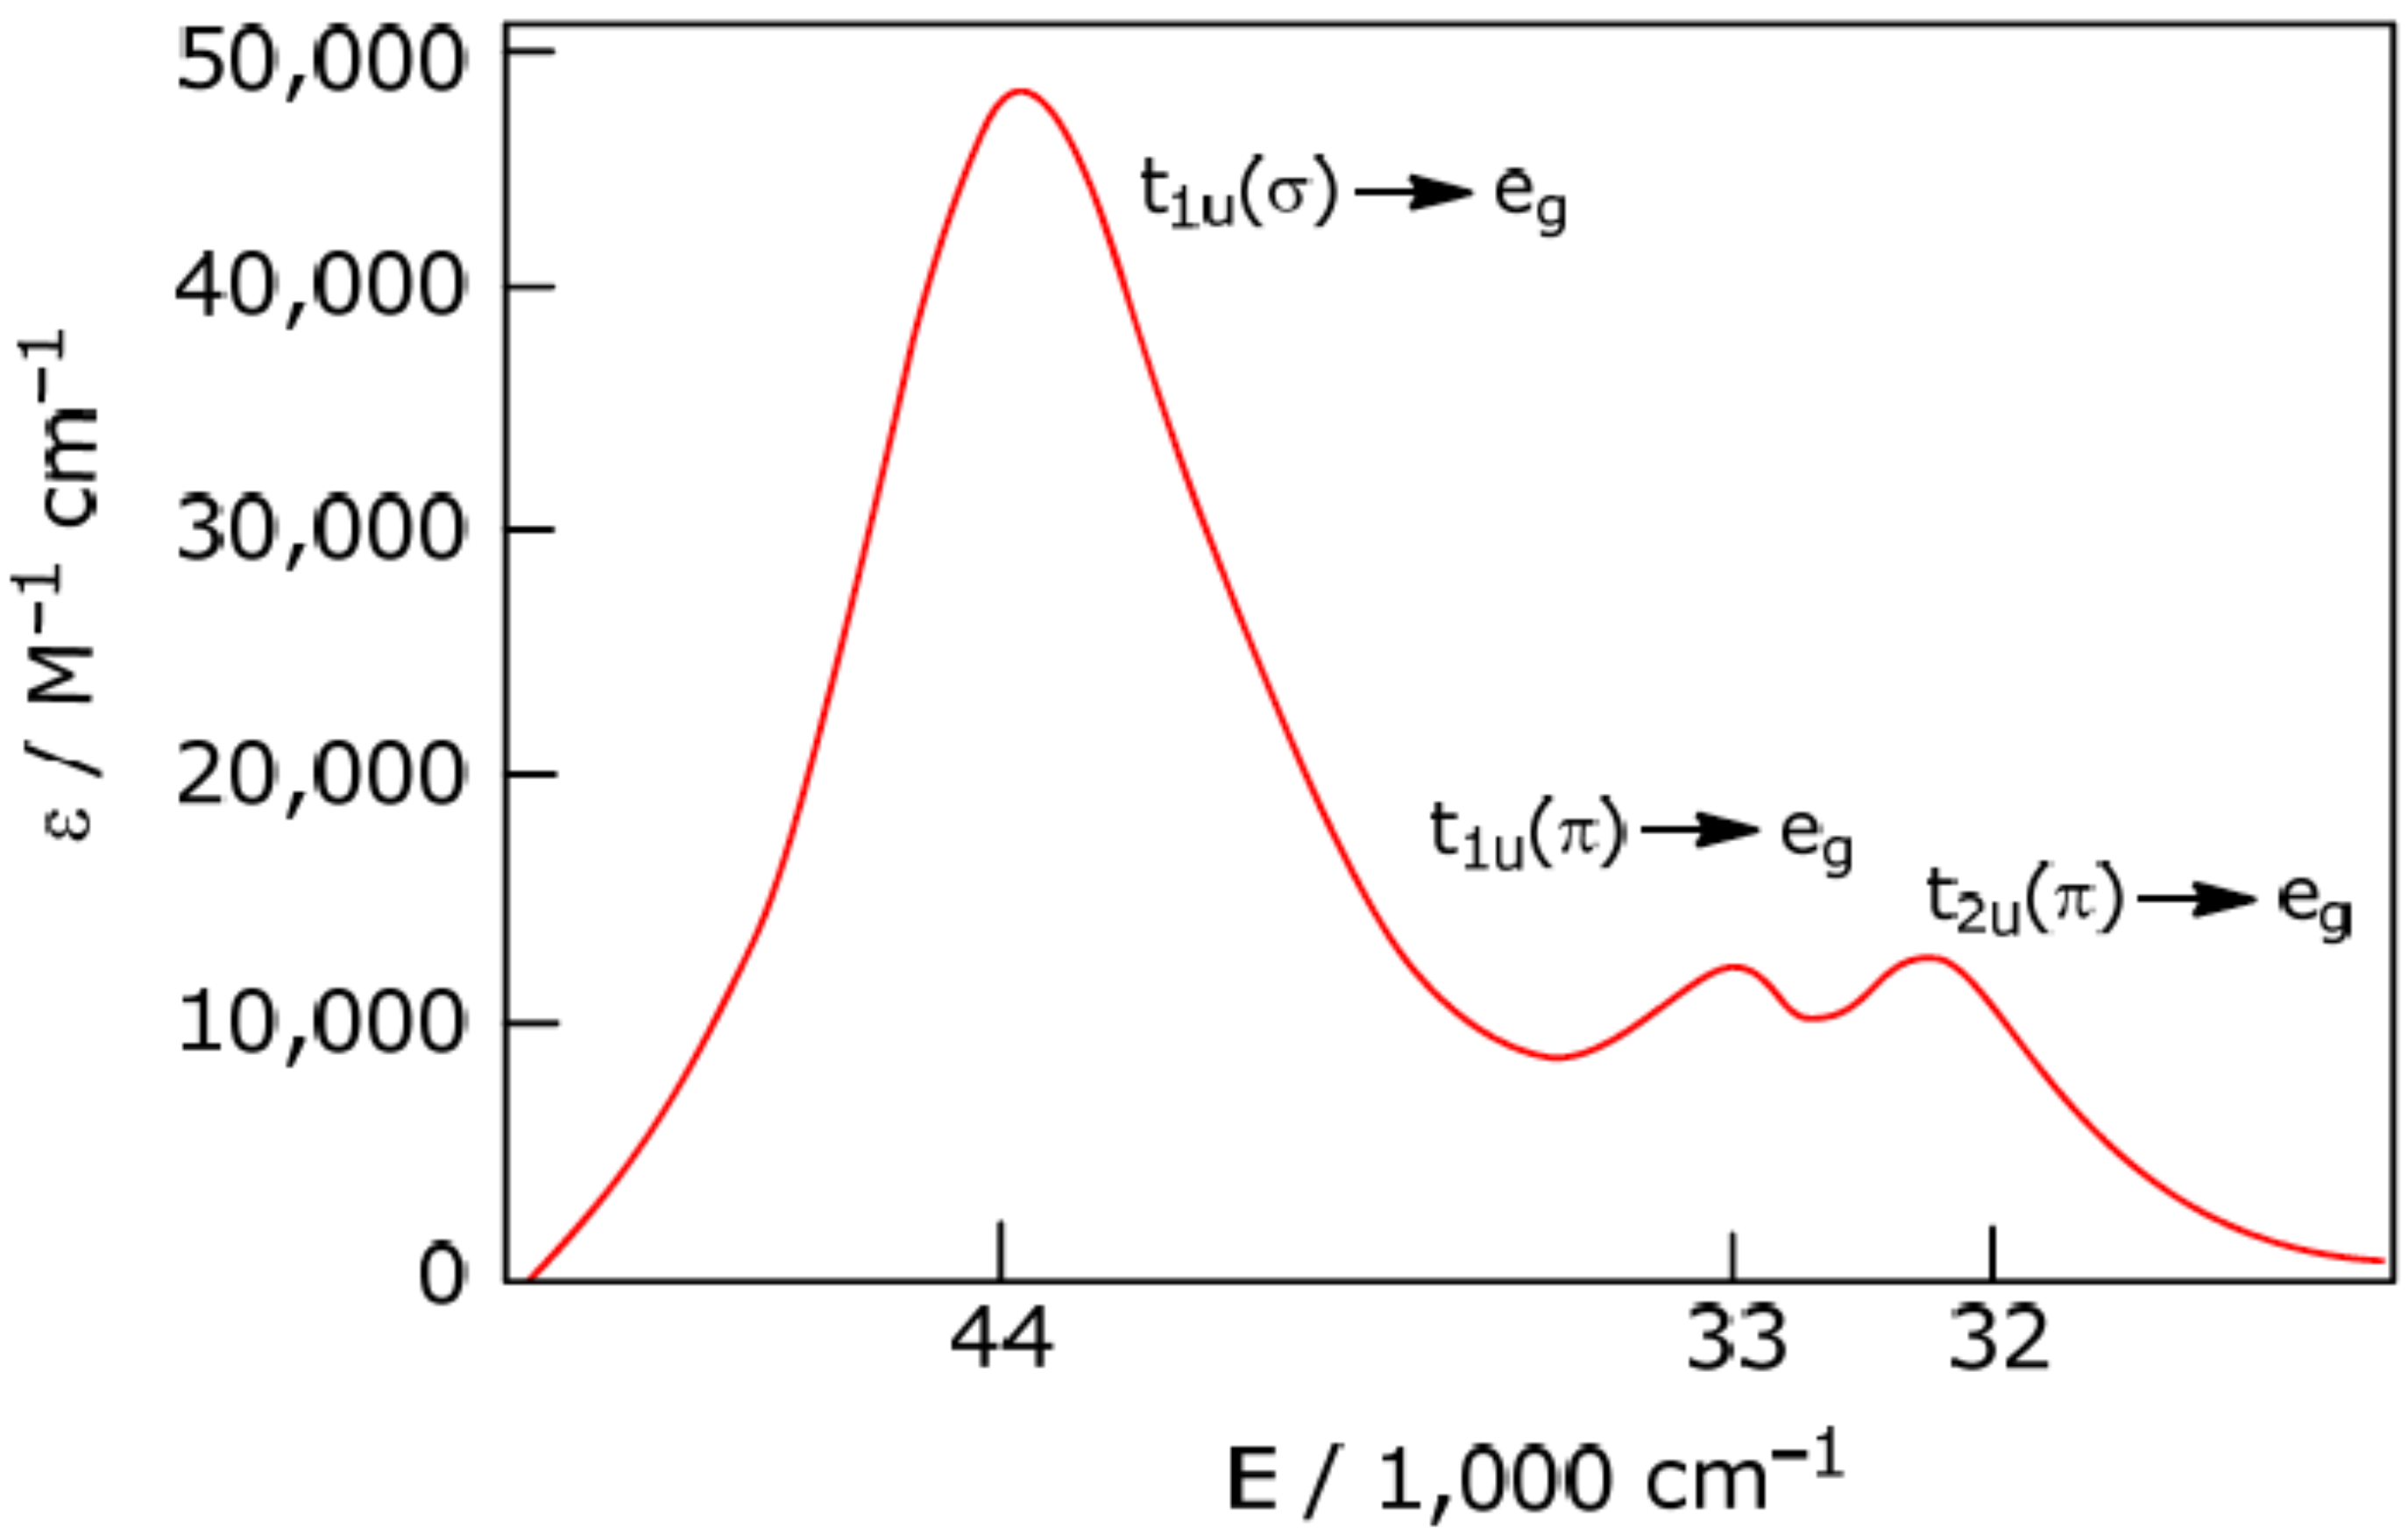
\includegraphics[width=\linewidth]{../ExtFiles/LMCTa.png}
            \caption{Spectrum.}
            \label{fig:LMCTa}
        \end{subfigure}
        \begin{subfigure}[b]{0.28\linewidth}
            \centering
            \begin{tikzpicture}
                \draw [densely dashed]
                    (0,0) -- ++(0:1)
                    (0,0) -- ++(45:1)
                    (0,0) -- ++(90:1)
                    (0,0) -- ++(180:1)
                    (0,0) -- ++(-90:1)
                ;
    
                \filldraw [semithick,fill=white,rotate=45] (0,0)
                    to[out=0,in=0,out looseness=0.5,in looseness=1.5] ++(0,0.65)
                    to[out=180,in=180,out looseness=1.5,in looseness=0.5] cycle
                ;
                \filldraw [semithick,fill=white,rotate=-135] (0,0)
                    to[out=0,in=0,out looseness=0.5,in looseness=1.5] ++(0,0.65)
                    to[out=180,in=180,out looseness=1.5,in looseness=0.5] cycle
                ;
                \filldraw [semithick,fill=grz,rotate=-45] (0,0)
                    to[out=0,in=0,out looseness=0.5,in looseness=1.5] ++(0,0.65)
                    to[out=180,in=180,out looseness=1.5,in looseness=0.5] cycle
                ;
                \filldraw [semithick,fill=grz,rotate=135] (0,0)
                    to[out=0,in=0,out looseness=0.5,in looseness=1.5] ++(0,0.65)
                    to[out=180,in=180,out looseness=1.5,in looseness=0.5] cycle
                ;
    
                \draw [densely dashed] (0,0) -- ++(-135:1);
    
                \filldraw [semithick,fill=white,rotate around={90:(0,1)}] (0,1)
                    to[out=0,in=0,out looseness=0.5] ++(0,0.65)
                    to[out=180,in=180,in looseness=0.5] cycle
                ;
                \filldraw [semithick,fill=grz,rotate around={-90:(0,1)}] (0,1)
                    to[out=0,in=0,out looseness=0.5] ++(0,0.65)
                    to[out=180,in=180,in looseness=0.5] cycle
                ;
    
                \draw [semithick,-stealth] (-0.75,1) to[bend right=70] (-0.6,0.5);
            \end{tikzpicture}
            \caption{$\pi$-donation.}
            \label{fig:LMCTb}
        \end{subfigure}
        \begin{subfigure}[b]{0.3\linewidth}
            \centering
            \begin{tikzpicture}[
                da/.pic={\node{$\upharpoonleft\hspace{-1mm}\downharpoonright$};}
            ]
                \Large
                \draw [ultra thick]
                    (-0.55,2)    --         ++(0.5,0) ++(0.1,0) --         ++(0.5,0)
                    (-0.85,1.5)  -- pic{da} ++(0.5,0) ++(0.1,0) -- pic{da} ++(0.5,0) ++(0.1,0) -- pic{da} ++(0.5,0)
                    (-0.85,0.3)  -- pic{da} ++(0.5,0) ++(0.1,0) -- pic{da} ++(0.5,0) ++(0.1,0) -- pic{da} ++(0.5,0)
                    (-0.85,-0.3) -- pic{da} ++(0.5,0) ++(0.1,0) -- pic{da} ++(0.5,0) ++(0.1,0) -- pic{da} ++(0.5,0)
                    (-0.85,-1.2) -- pic{da} ++(0.5,0) ++(0.1,0) -- pic{da} ++(0.5,0) ++(0.1,0) -- pic{da} ++(0.5,0)
                    (-0.85,-1.8) -- pic{da} ++(0.5,0) ++(0.1,0) -- pic{da} ++(0.5,0) ++(0.1,0) -- pic{da} ++(0.5,0)
                ;
    
                \footnotesize
                \node [right] at (1,2)    {\ce{M-L\sigma^*}, $e_g$};
                \node [right] at (1,1.5)  {\ce{M-L\pi^*}, $t_{2g}$};
                \node [right] at (1,0)    {$t_{1u}(\pi)$ / $t_{2u}(\pi)$};
                \node [right] at (1,-1.5) {$t_{1u}(\sigma)$};

                \draw [-stealth] (-1,0) -- ++(0,2);
                \draw [-stealth] (-1.3,-1.5) -- ++(0,3.5);
    
                % \path (-3.1,0) -- (3.1,0);
            \end{tikzpicture}
            \caption{MO diagram.}
            \label{fig:LMCTc}
        \end{subfigure}
        \caption{LMCT dynamics.}
        \label{fig:LMCT}
    \end{figure}
    \begin{itemize}
        \item Figure \ref{fig:LMCTa} depicts the spectrum for \ce{[PtBr6]^2-}.
        \item All ligands are $\pi$-donating.
        \item If we think about the MO parentage (ligand $p$-orbital and metal $d$-orbital), we can have a charge transfer from the ligand to the metal because of the MO diagram (see Figure \ref{fig:LMCTb}; Wuttig appears to draw it as antibonding?? Reversed $p$-orbital sign??).
        \item All of the orbitals below the frontier $t_{2g}$ \ce{M-L\pi^*} set are completely occupied, and what we're observing is the transition from those lower-lying orbitals, up, as illustrated in Figure \ref{fig:LMCTc}.
        \begin{itemize}
            \item Notice that the transitions in this MO diagram exactly mirror those in the spectrum in Figure \ref{fig:LMCTa}.
            \item Possible inconsistency??: Figure \ref{fig:LMCTa} is consistent with Figure \ref{fig:LMCTc}, but according to Figure \ref{fig:MOsML6pi}, $t_{2u}(\pi)$ should be degenerate with $t_{1g}(\pi)$, not $t_{1u}(\pi)$. Overall actually, the orbitals don't look entirely consistent. What modifications are we making?
        \end{itemize}
        \item LMCT is Laporte allowed because the ligand $p$ orbital (ground state) is ungerade and the metal $d$ orbital (excited state) is gerade. Mathematically,
        \begin{equation*}
            g_\text{es}\times u\times u_\text{gs} = g
        \end{equation*}
        \item Molar extinction coefficients are \emph{very} high (tens of thousands vs. single-digit $d$-$d$ transitions).
    \end{itemize}
    \item Question: Rank the energy of the LMCT transitions among \ce{[OsBr6]^2-}, \ce{[OsCl6]^2-}, and \ce{[OsI6]^2-}.
    \begin{itemize}
        \item Largest electronegativity (chloride) leads to the largest LMCT transition; smallest leads to smallest (iodide).
        \item This is because larger electronegativity leads to lower bonding orbitals and thus a higher energy jump up to the frontier orbitals.
    \end{itemize}
    \item MLCT transitions.
    \begin{figure}[h!]
        \centering
        \begin{subfigure}[b]{0.4\linewidth}
            \centering
            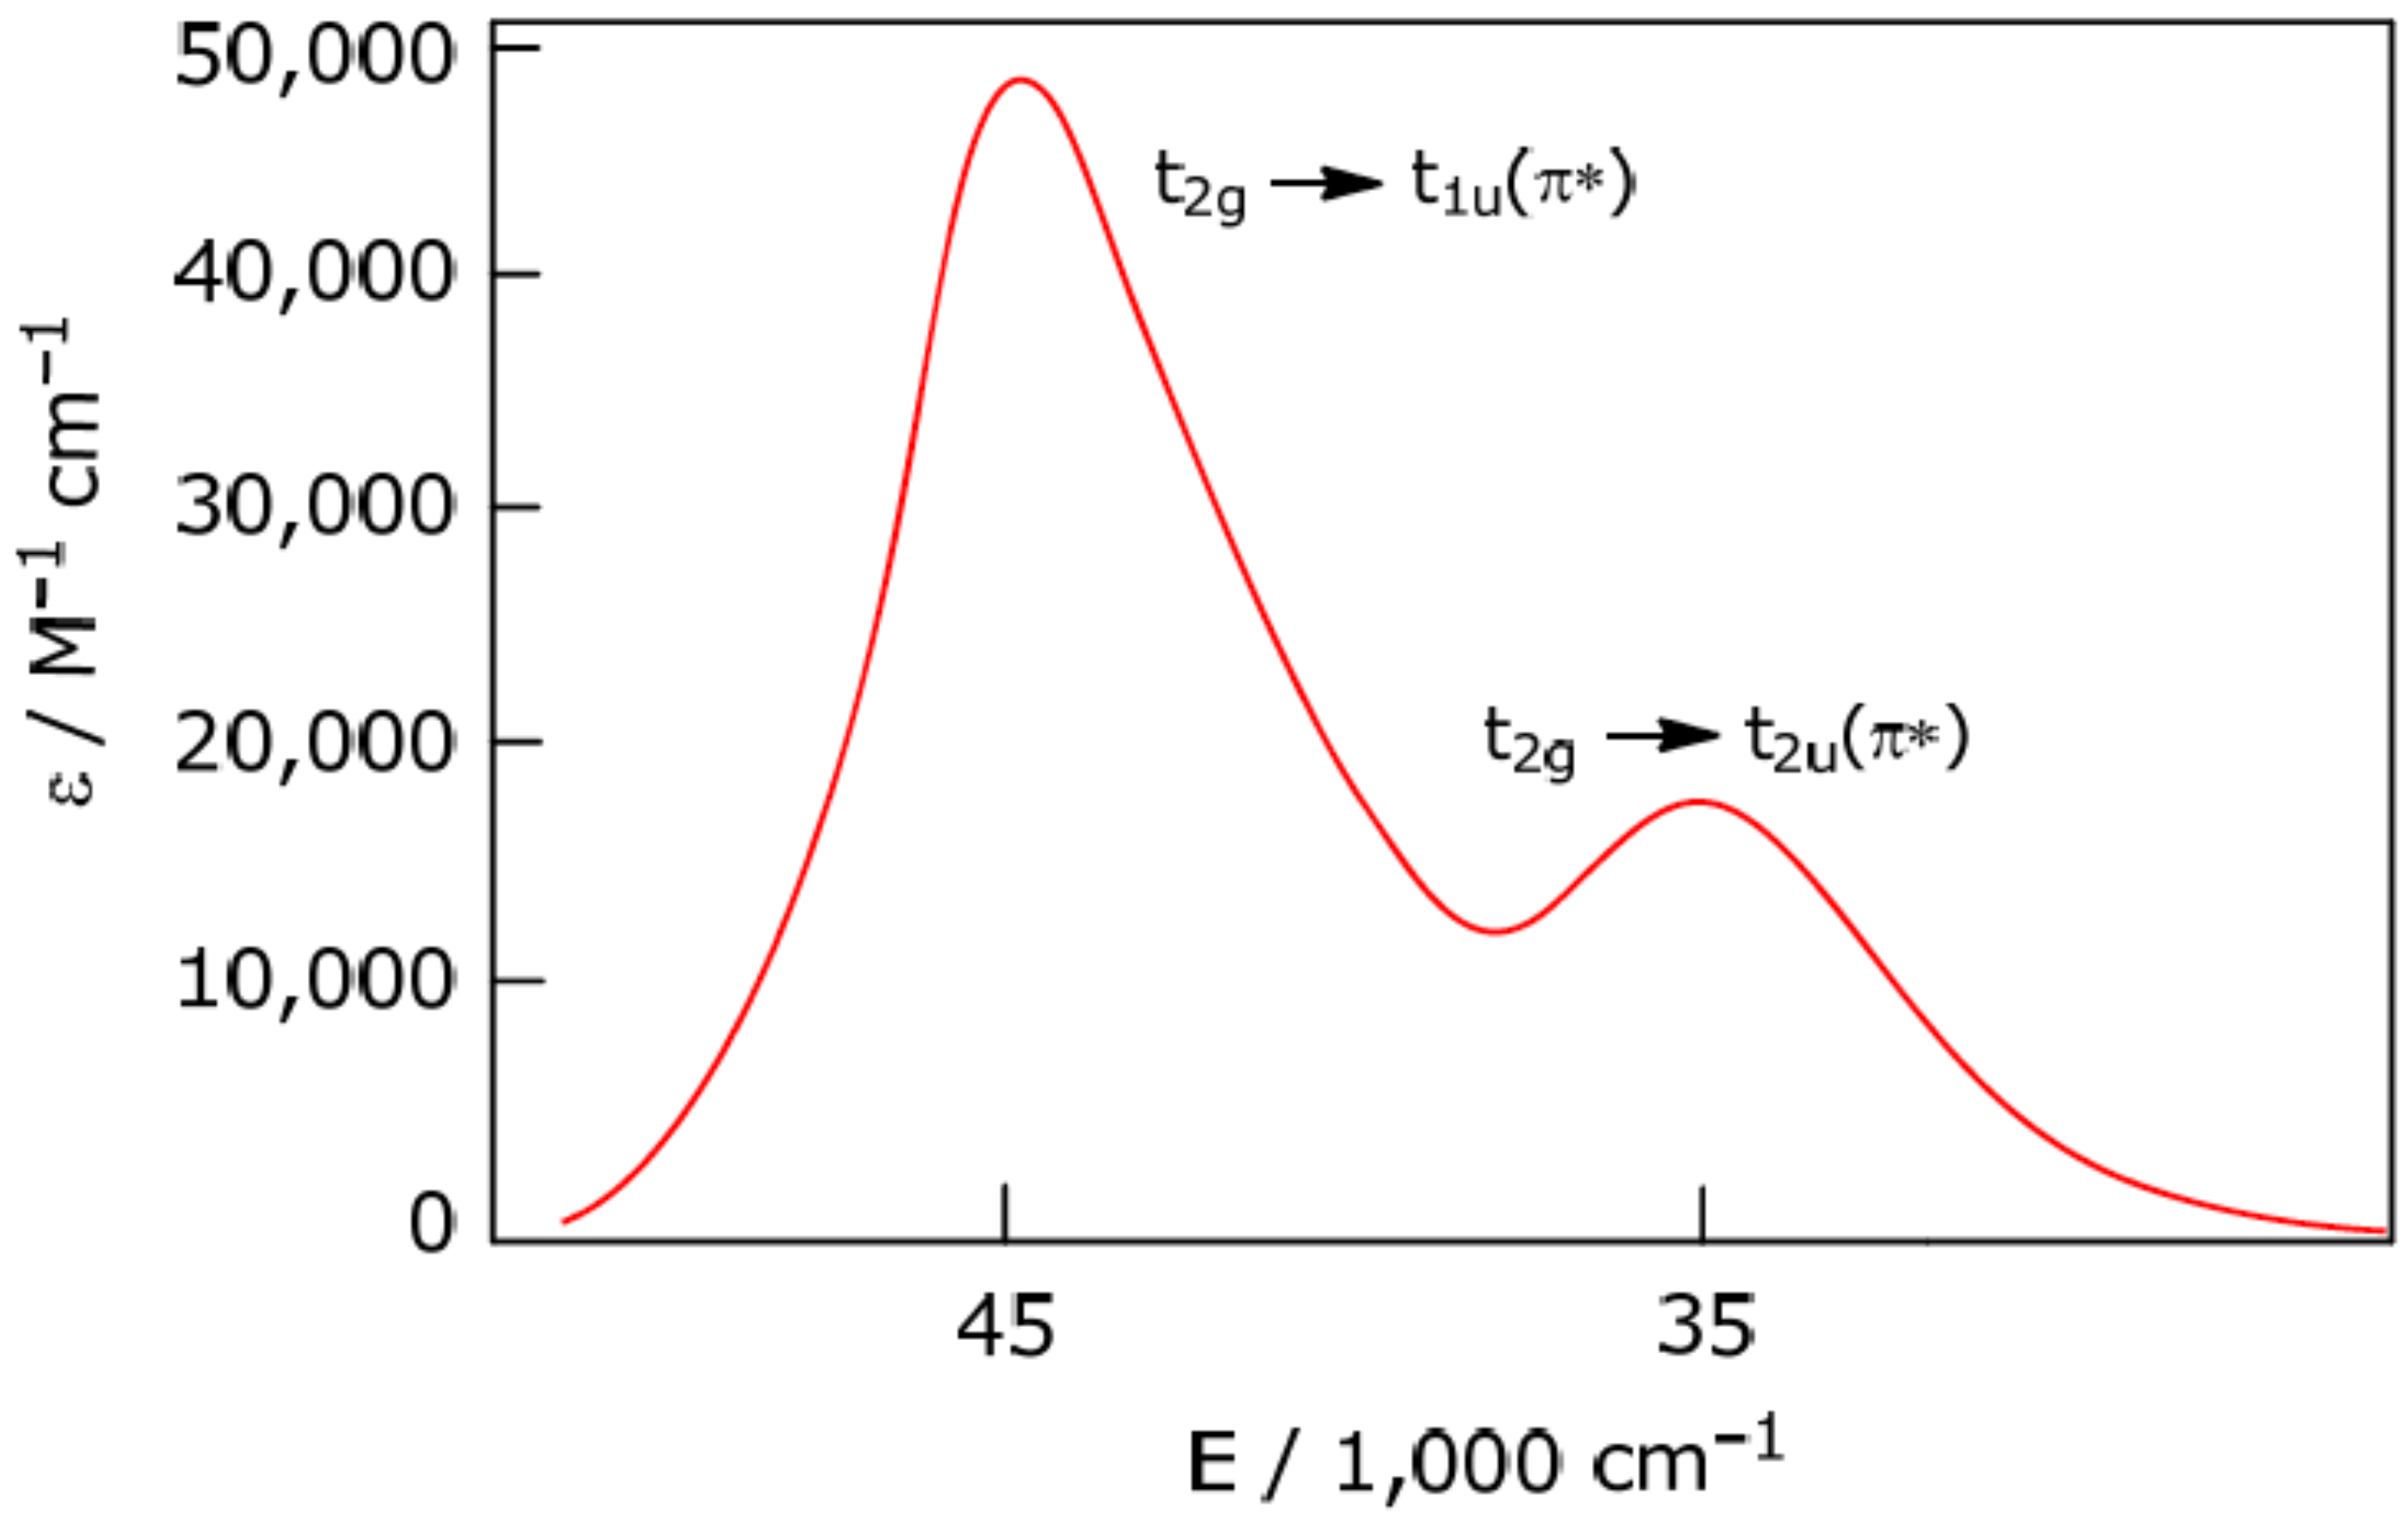
\includegraphics[width=\linewidth]{../ExtFiles/MLCTa.png}
            \caption{Spectrum.}
            \label{fig:MLCTa}
        \end{subfigure}
        \begin{subfigure}[b]{0.28\linewidth}
            \centering
            \begin{tikzpicture}
                \draw [densely dashed]
                    (0,0) -- ++(0:1)
                    (0,0) -- ++(45:1)
                    (0,0) -- ++(90:1)
                    (0,0) -- ++(180:1)
                    (0,0) -- ++(-90:1)
                ;
    
                \filldraw [semithick,fill=white,rotate=45] (0,0)
                    to[out=0,in=0,out looseness=0.5,in looseness=1.5] ++(0,0.65)
                    to[out=180,in=180,out looseness=1.5,in looseness=0.5] cycle
                ;
                \filldraw [semithick,fill=white,rotate=-135] (0,0)
                    to[out=0,in=0,out looseness=0.5,in looseness=1.5] ++(0,0.65)
                    to[out=180,in=180,out looseness=1.5,in looseness=0.5] cycle
                ;
                \filldraw [semithick,fill=grz,rotate=-45] (0,0)
                    to[out=0,in=0,out looseness=0.5,in looseness=1.5] ++(0,0.65)
                    to[out=180,in=180,out looseness=1.5,in looseness=0.5] cycle
                ;
                \filldraw [semithick,fill=grz,rotate=135] (0,0)
                    to[out=0,in=0,out looseness=0.5,in looseness=1.5] ++(0,0.65)
                    to[out=180,in=180,out looseness=1.5,in looseness=0.5] cycle
                ;
    
                \draw [densely dashed] (0,0) -- ++(-135:1);
    
                \filldraw [semithick,fill=white,rotate around={90:(0,1)}] (0,1)
                    to[out=0,in=0,out looseness=0.5] ++(0,0.65)
                    to[out=180,in=180,in looseness=0.5] cycle
                ;
                \filldraw [semithick,fill=grz,rotate around={-90:(0,1)}] (0,1)
                    to[out=0,in=0,out looseness=0.5] ++(0,0.65)
                    to[out=180,in=180,in looseness=0.5] cycle
                ;
                \filldraw [semithick,fill=white,rotate around={-90:(0,1.4)}] (0,1.4)
                    to[out=0,in=0,out looseness=0.5] ++(0,0.65)
                    to[out=180,in=180,in looseness=0.5] cycle
                ;
                \filldraw [semithick,fill=grz,rotate around={90:(0,1.4)}] (0,1.4)
                    to[out=0,in=0,out looseness=0.5] ++(0,0.65)
                    to[out=180,in=180,in looseness=0.5] cycle
                ;
    
                \draw [semithick,stealth-] (0.75,1) to[bend left=70] (0.6,0.5);
            \end{tikzpicture}
            \caption{$\pi$-acceptance.}
            \label{fig:MLCTb}
        \end{subfigure}
        \begin{subfigure}[b]{0.3\linewidth}
            \centering
            \begin{tikzpicture}[
                da/.pic={\node{$\upharpoonleft\hspace{-1mm}\downharpoonright$};}
            ]
                \Large
                \draw [ultra thick]
                    (-0.85,1)    --         ++(0.5,0) ++(0.1,0) --         ++(0.5,0) ++(0.1,0) --         ++(0.5,0)
                    (-0.85,0.5)  --         ++(0.5,0) ++(0.1,0) --         ++(0.5,0) ++(0.1,0) --         ++(0.5,0)
                    (-0.55,-1)   --         ++(0.5,0) ++(0.1,0) --         ++(0.5,0)
                    (-0.85,-1.5) -- pic{da} ++(0.5,0) ++(0.1,0) -- pic{da} ++(0.5,0) ++(0.1,0) -- pic{da} ++(0.5,0)
                ;
    
                \footnotesize
                \node [right] at (1,1)  {$t_{1u}(\pi^*)$};
                \node [right] at (1,0.5)  {$t_{2u}(\pi^*)$};
                \node [right] at (1,-1)   {\ce{M-L\sigma^*}, $e_g$};
                \node [right] at (1,-1.5) {\ce{M-L\pi}, $t_{2g}$};

                \draw [-stealth] (-1,-1.5)   -- ++(0,2);
                \draw [-stealth] (-1.3,-1.5) -- ++(0,2.5);
    
                \path (-3.1,0) -- (3.1,0);
            \end{tikzpicture}
            \caption{MO diagram.}
            \label{fig:MLCTc}
        \end{subfigure}
        \caption{MLCT dynamics.}
        \label{fig:MLCT}
    \end{figure}
    \begin{itemize}
        \item Figure \ref{fig:MLCTa} depicts the spectrum for \ce{[Cr(CO)6]^3+}.
        \item All ligands are $\pi$-accepting
        \item Once again, we get very large extinction coefficients, so we must be relaxing the Laporte selection rule.
        \begin{itemize}
            \item Laporte allowed due to transitions occurring from gerade ground states to ungerade excited states.
        \end{itemize}
        \item We excite electrons from the metal to the ligand in the MO diagram, resulting in two transitions in both the diagram (Figure \ref{fig:MLCTc}) and the spectrum (Figure \ref{fig:MLCTa}).
    \end{itemize}
    \item Technological applications of MLCT.
    \begin{itemize}
        \item The transitions are so allowed that we get a lot of applications.
    \end{itemize}
    \item The Gr\"{a}tzel Cell (by Michael Gr\"{a}tzel at EPFL). You can't store energy, but you can take light and generate an electric current.
    \begin{figure}[h!]
        \centering
        \begin{subfigure}[b]{0.49\linewidth}
            \centering
            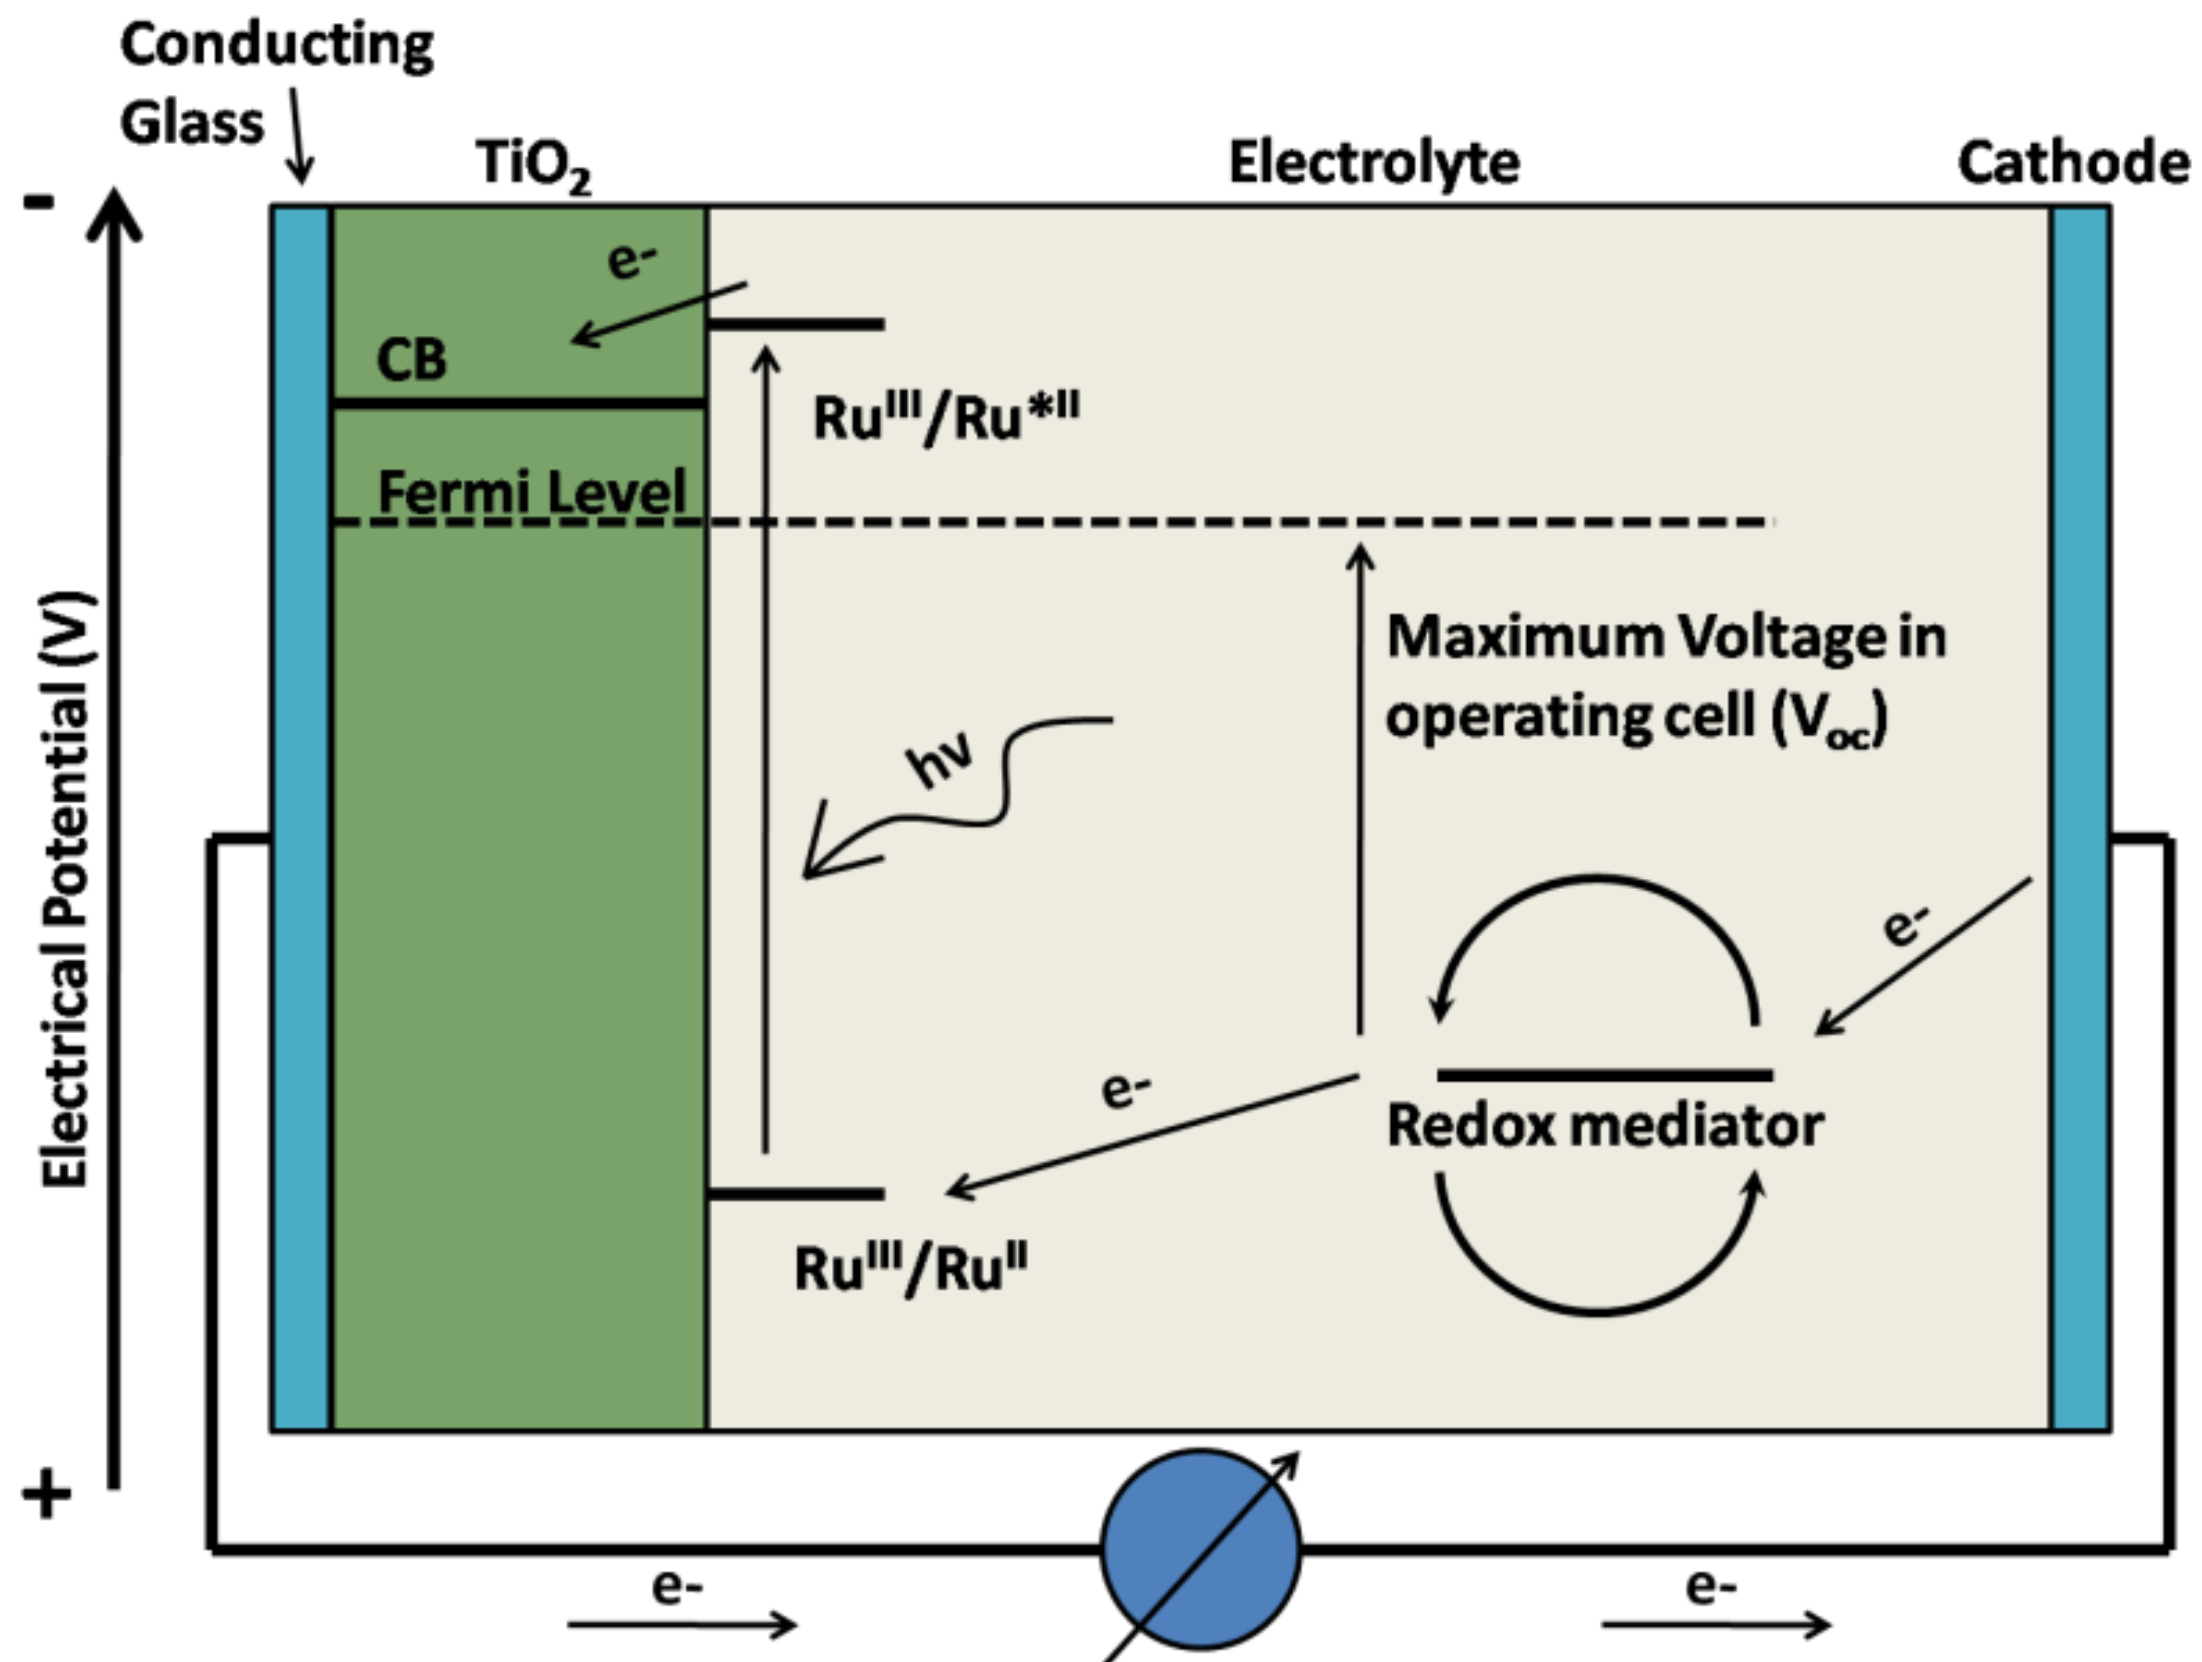
\includegraphics[width=0.9\linewidth]{../ExtFiles/GratzelCella.png}
            \caption{Overall design.}
            \label{fig:GratzelCella}
        \end{subfigure}
        \begin{subfigure}[b]{0.49\linewidth}
            \centering
            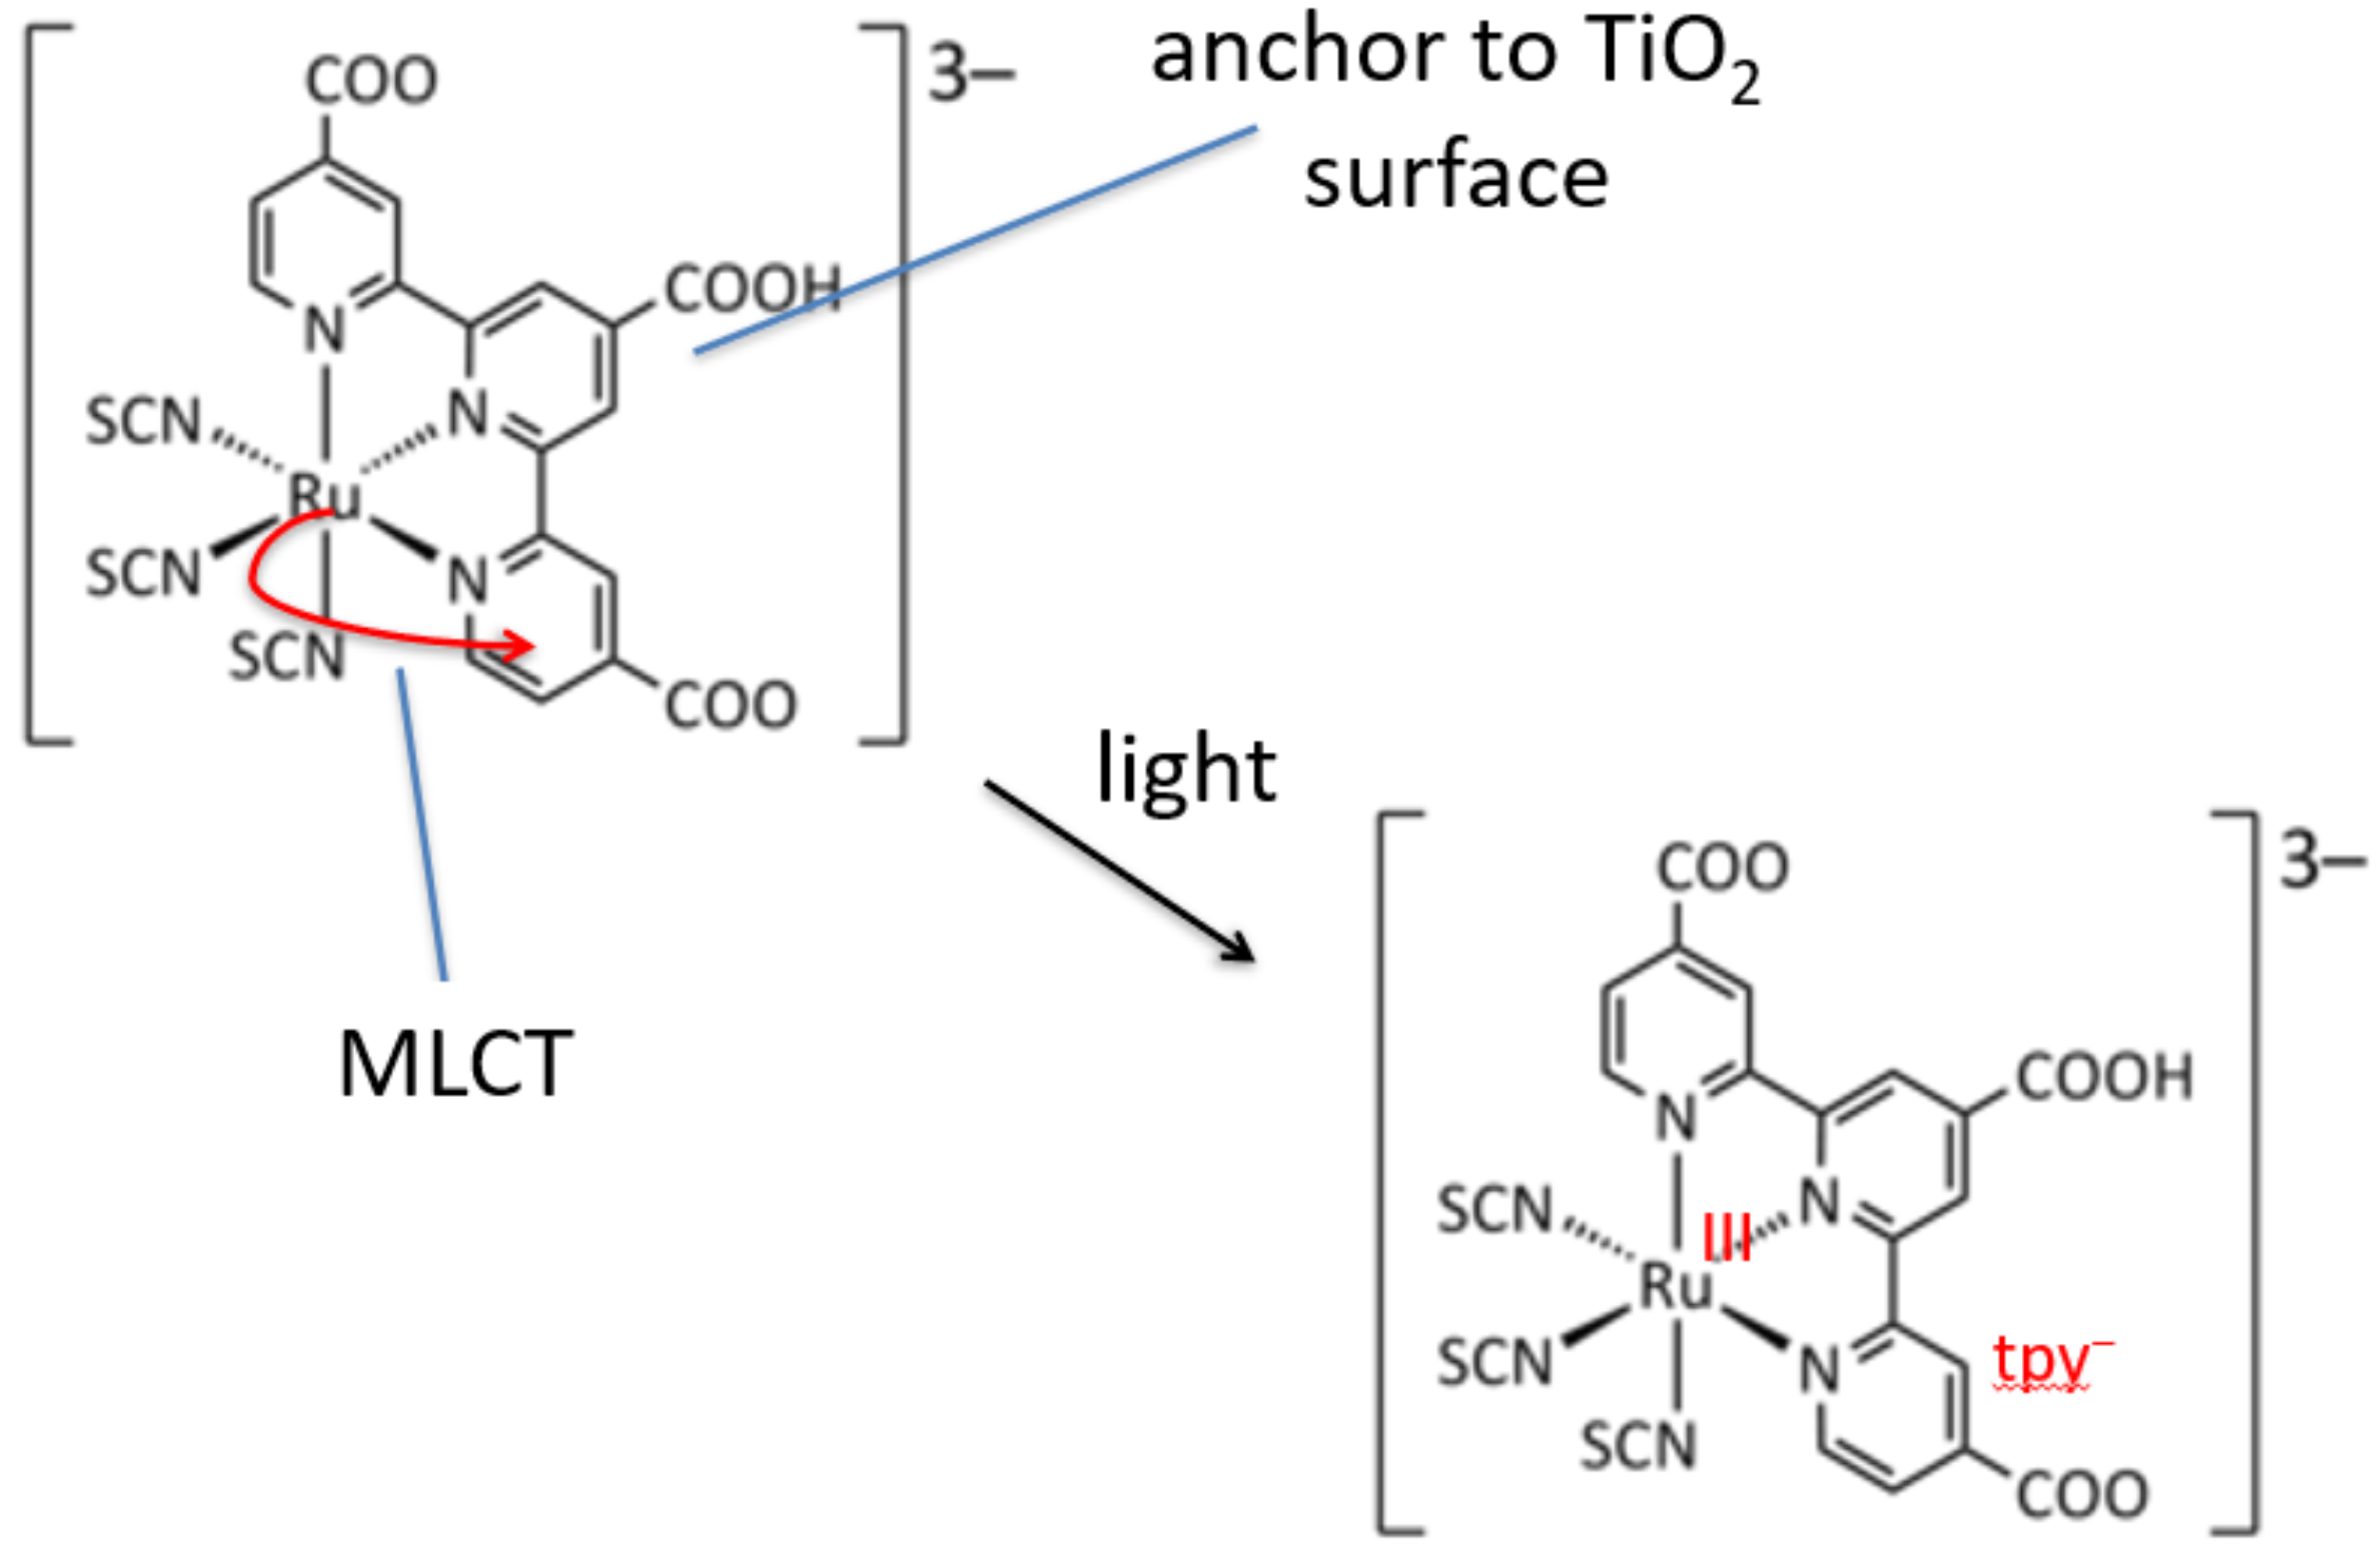
\includegraphics[width=0.9\linewidth]{../ExtFiles/GratzelCellb.png}
            \caption{MLCT step.}
            \label{fig:GratzelCellb}
        \end{subfigure}
        \caption{Gr\"{a}tzel Cell mechanism.}
        \label{fig:GratzelCell}
    \end{figure}
    \begin{itemize}
        \item A bit like artificial photosynthesis. We can't generate fuel like in a fuel cell, but we can generate current.
        \item Uses a \ce{Ru(SCN)3L} complex. Experimentally, this molecule has a very deep MLCT charge transfer band, allowing it to absorb into the red and IR spectrum (needed for direct sunlight to electricity conversion).
        \item The compound is anchored onto a \ce{TiO2} (semiconducting) surface. The band gap is about \SI{3}{\electronvolt}. The \textbf{conduction band} (LUMO for an extended solid) is poised at a level such that when you photoexcite \ce{Ru^{II}}, oxidizing via MLCT \ce{Ru^{II} -> Ru^{III}} and reducing the \ce{tpy} ligand, you get an electron in an orbital (on \ce{tpy-}) that is higher than the \ce{TiO2} conduction band.
        \item Thus, you can dump the electron into \ce{TiO2}.
        \item \ce{TiO2} is connected to a conducting glass (usually fluorine-doped tin oxide) from which you can harvest the electron and use it for electricity.
        \item An additional redox mediator is used in solution to harvest electrons at a cathode and regenerate \ce{Ru^2+}; this is essential in order to be able to do the same thing again (think salt bridge). The mediator goes from
        \begin{equation*}
            \ce{I3- -> 3I-}
        \end{equation*}
        \item The lifetimes aren't that great.
        \item Selling point is that it is made out of very cheap materials, and is efficient because it makes use of very highly allowed MLCTs.
    \end{itemize}
    \item Photoredox catalysis.
    \begin{figure}[h!]
        \centering
        \begin{subfigure}[b]{0.3\linewidth}
            \centering
            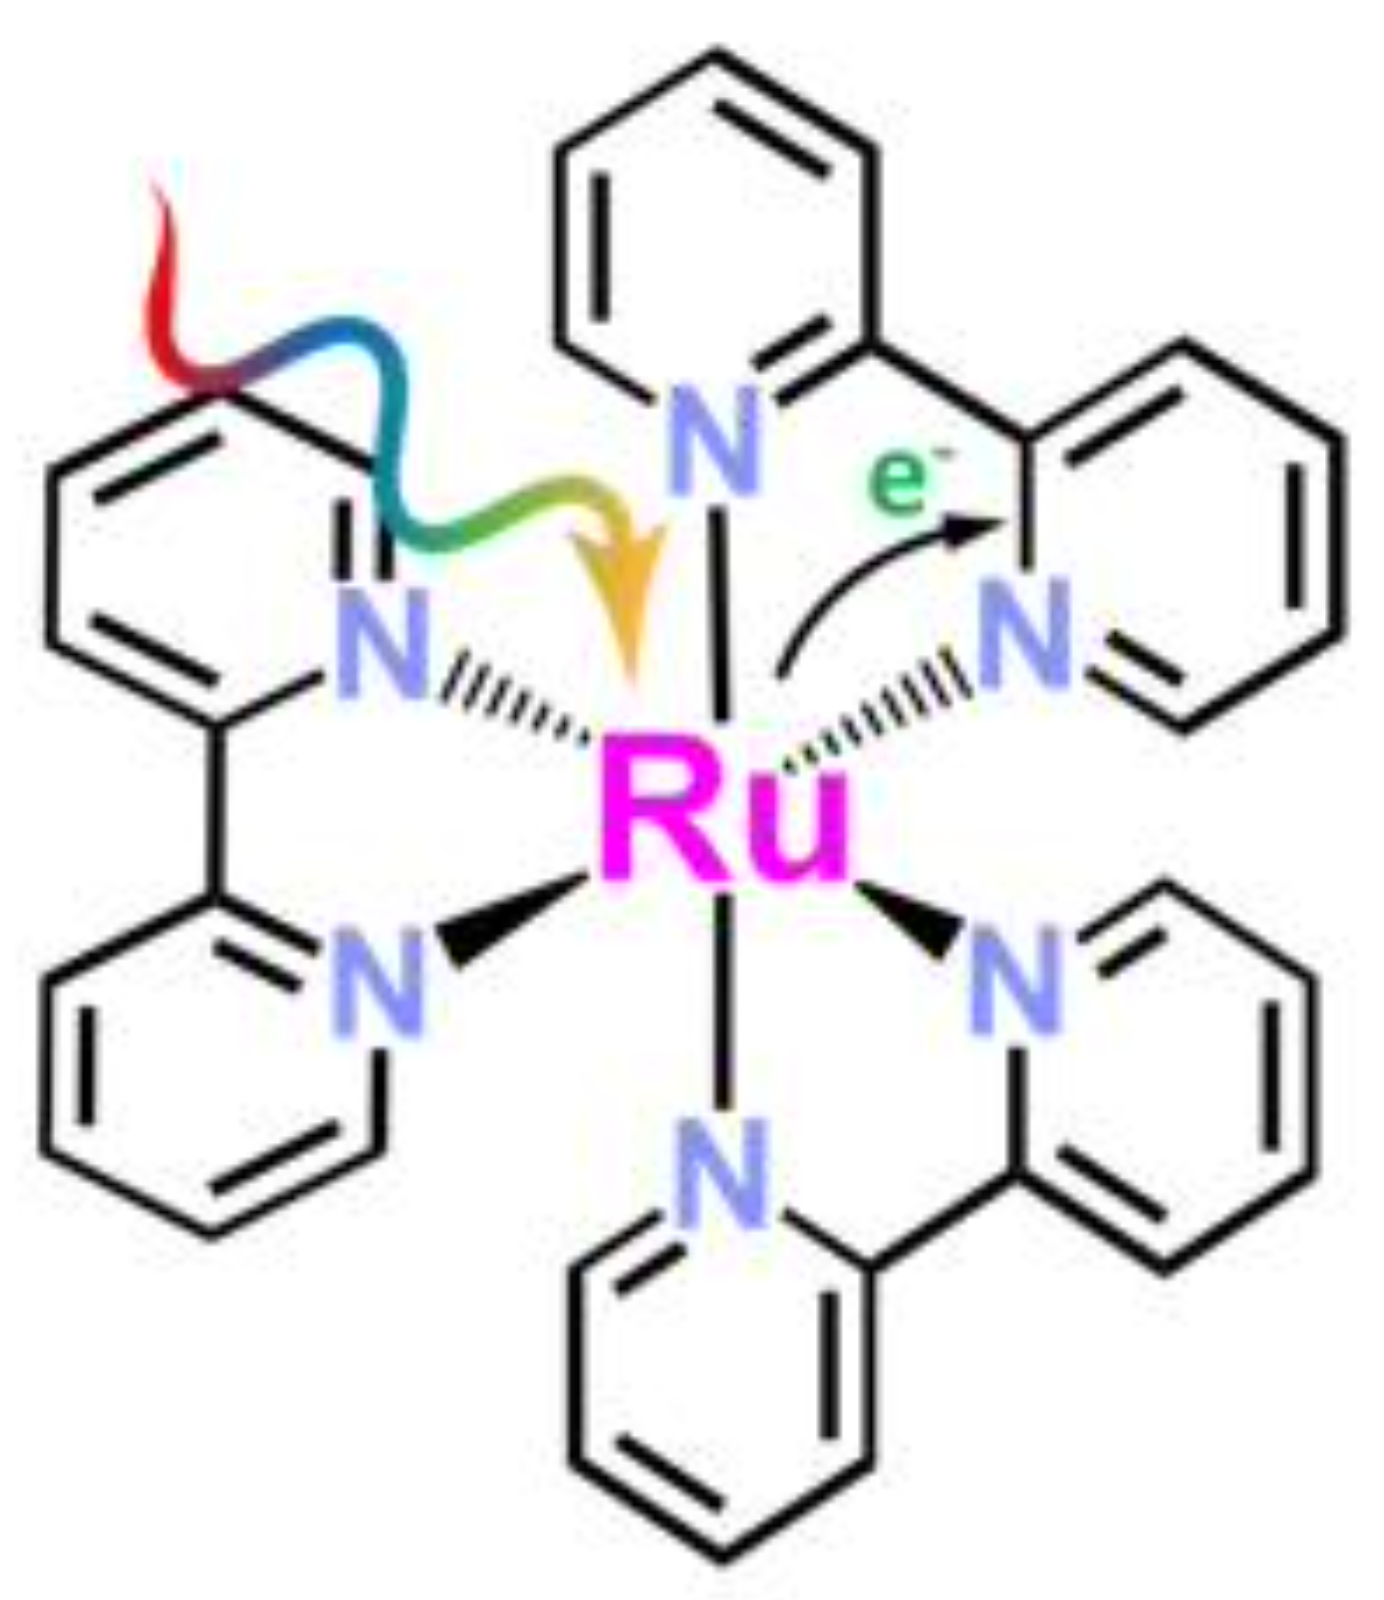
\includegraphics[width=0.7\linewidth]{../ExtFiles/photoredoxCatala.png}
            \caption{\ce{[Ru(bpy)3]^2+} light absorption.}
            \label{fig:photoredoxCatala}
        \end{subfigure}
        \begin{subfigure}[b]{0.68\linewidth}
            \centering
            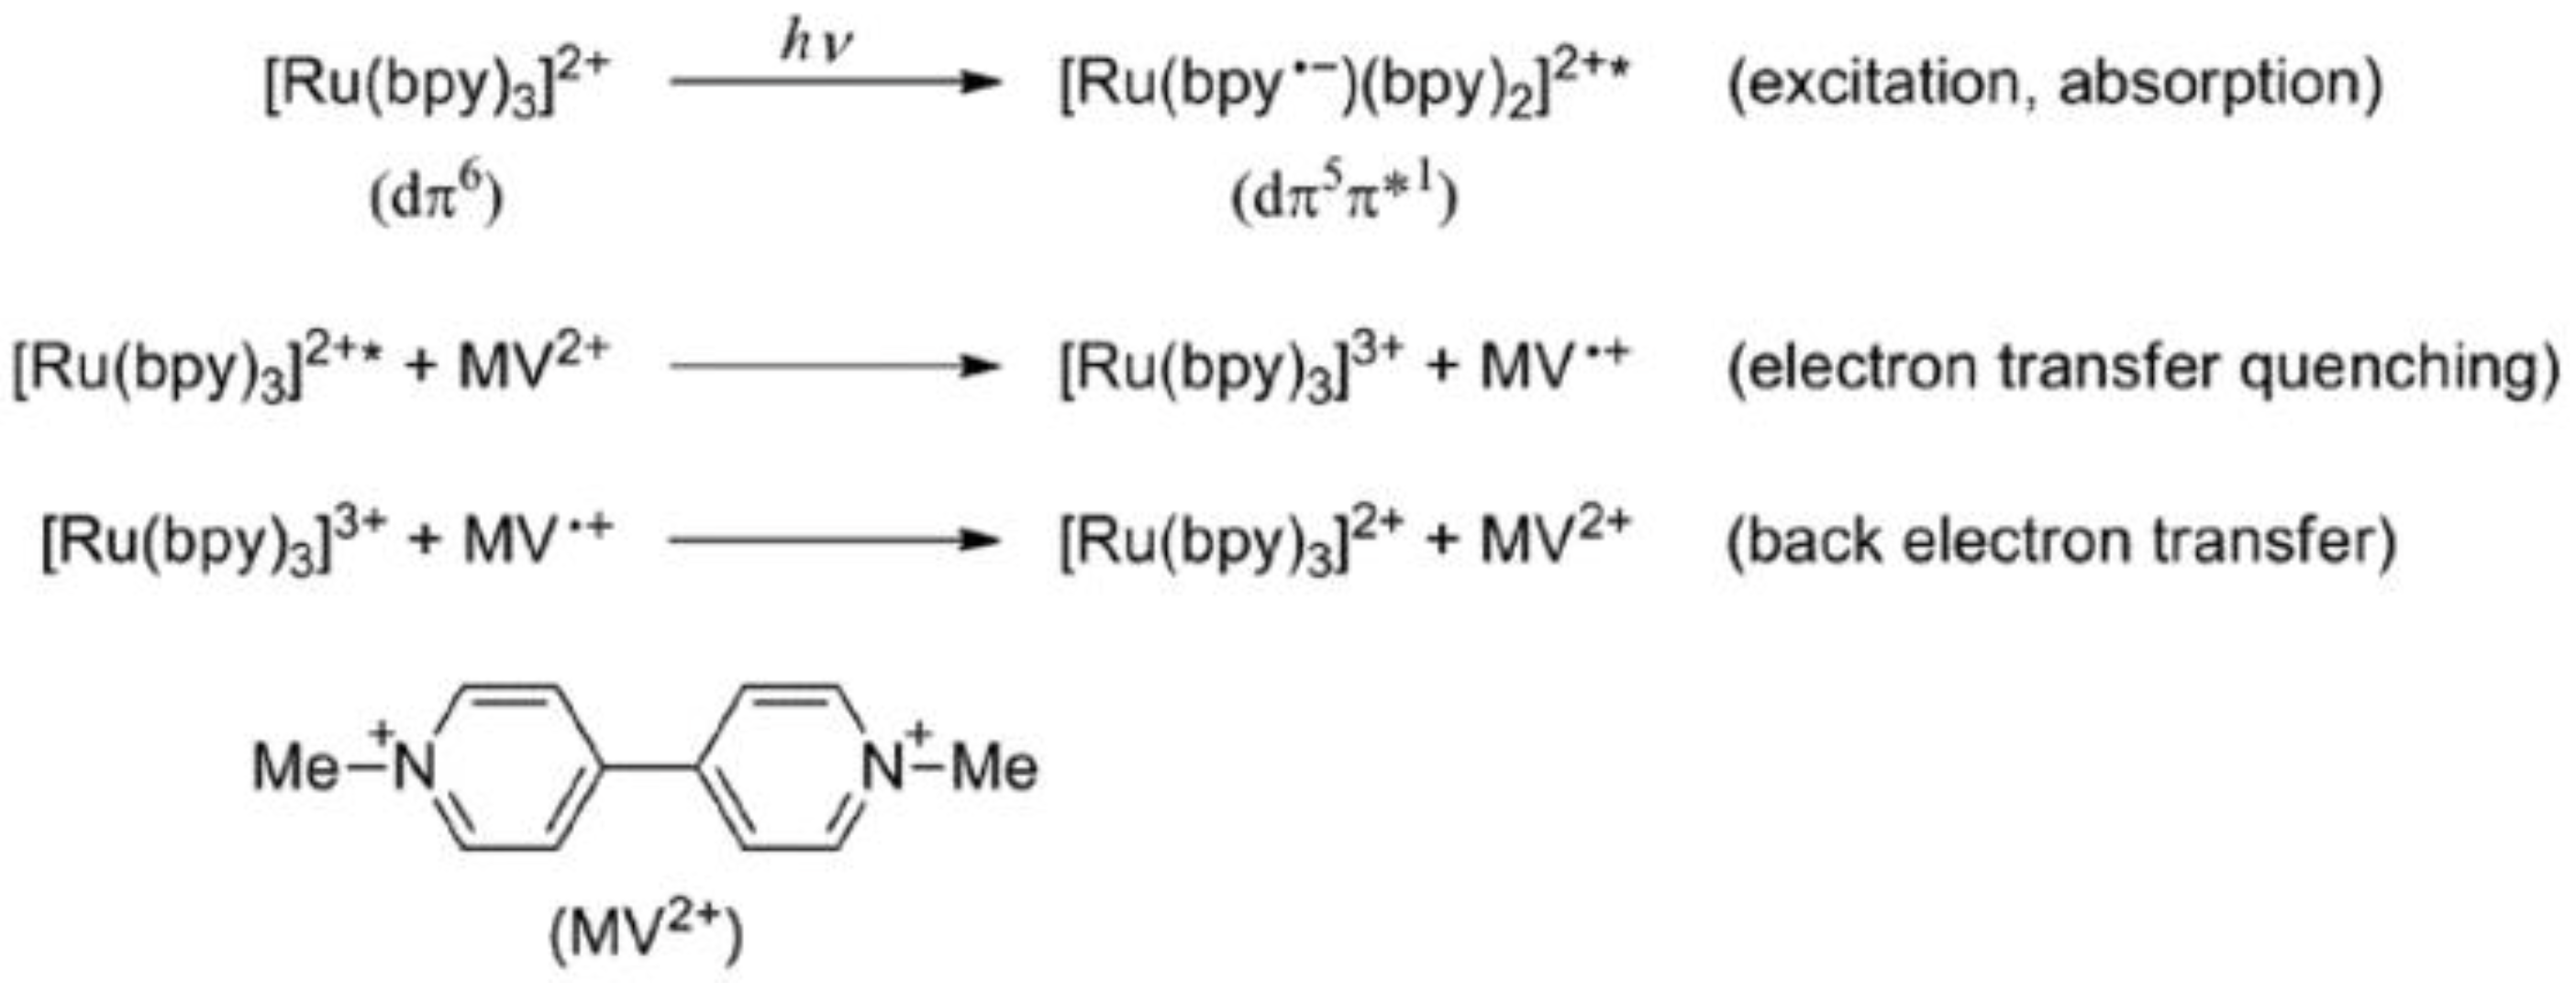
\includegraphics[width=0.9\linewidth]{../ExtFiles/photoredoxCatalb.png}
            \caption{Discovery mechanism: Quenching with \ce{MV^2+}.}
            \label{fig:photoredoxCatalb}
        \end{subfigure}
        \caption{Photoredox catalysis.}
        \label{fig:photoredoxCatal}
    \end{figure}
    \begin{itemize}
        \item Organic chemists have usurped it for catalysis, but it all came from inorganic chemistry.
        \item Whitten and Meyer established that \ce{Ru(bpy)3^2+} complexes have charge transfer processes, that the excited electron can reduce various organic compounds, and that the hole left behind can be refilled.
        \begin{equation*}
            \underbrace{\ce{[Ru(bpy)3]^2+}}_{d\pi^6} \ce{->[$h\nu$]} \underbrace{\ce{[Ru(bpy^{\cdot -})(bpy)2]^{2+*}}}_{d\pi^5{\pi^*}^1}
        \end{equation*}
        \begin{itemize}
            \item Discovered this by quenching the reaction with methyl viologen (\ce{MV^2+}).
        \end{itemize}
        \item The seminal papers are the \textbf{Meyer papers}.
        \item We improve photoredox catalysis further by thinking about the relative energy levels between where the $d$ electrons are coming from and where they're going.
        \begin{itemize}
            \item To this end, people have put in tons of \ce{CF3} groups to make a more powerful reductant.
        \end{itemize}
    \end{itemize}
    \item \textbf{Meyer papers}: The two papers \textcite{bib:Meyer1974} and \textcite{bib:Meyer2013}.
\end{itemize}




\end{document}